\documentclass[journal]{IEEEtran}

\usepackage[utf8]{inputenc}
\usepackage{graphicx}
\usepackage{amsmath}
\usepackage{amssymb}
\usepackage{url}
\usepackage{booktabs}
\usepackage{xcolor}
\usepackage{hyperref}
\usepackage{tikz}
\usepackage{pgfplots}
\pgfplotsset{compat=1.18}

\begin{document}

\title{Mitigating Prompt Injection Attacks in LLM-Based Systems Using Multi-Layer Guardrails: Part III -- Evaluation Framework, Baselines, and Discussion}

\author{
    \IEEEauthorblockN{Your Name}
    \IEEEauthorblockA{\textit{Your Department} \\
    \textit{Your University or Organization}\\
    City, Country \\
    your.email@example.com}
}

\maketitle
\setcounter{page}{11}

\begin{abstract}
This third part defines a journal-grade evaluation plan for Gradril and frames the prototype for a full 15--20 page publication. It presents benchmark groups, baselines, metrics, graph templates, and an ablation strategy grounded in the actual codebase. It also discusses strengths, limitations, and the path required to transform the current prototype into a full empirical journal contribution.
\end{abstract}

\begin{IEEEkeywords}
LLM benchmarking, prompt-injection evaluation, ablation study, security metrics, experimental design.
\end{IEEEkeywords}

\section{Research Questions}
The evaluation of Gradril can be organized around the following research questions:
\begin{itemize}
    \item \textbf{RQ1:} How much does layered validation improve detection over regex-only filtering?
    \item \textbf{RQ2:} How much value does conversation-aware analysis add for staged attacks?
    \item \textbf{RQ3:} How effective is the semantic endpoint for paraphrased prompt injection?
    \item \textbf{RQ4:} What latency overhead is introduced by back-end validation?
    \item \textbf{RQ5:} How much does the code exfiltration detector improve protection in developer-assistant scenarios?
\end{itemize}

\section{Evaluation Design}
A journal-grade experimental setup should combine benign and malicious prompt sets. The benchmark should include at least five groups:
\begin{enumerate}
    \item benign development prompts,
    \item direct prompt-injection prompts,
    \item obfuscated or transformed prompts,
    \item multi-turn attack traces,
    \item code-exfiltration and secret-access prompts.
\end{enumerate}

Each sample should include a gold label for attack family, expected mitigation action, and whether the attack targets policy override, secret leakage, hidden prompt extraction, or downstream misuse.

\section{Baselines}
A meaningful journal study should compare Gradril against multiple baselines:
\begin{itemize}
    \item \textbf{B1: Regex-only local validators}
    \item \textbf{B2: Normalizer + regex}
    \item \textbf{B3: Back-end validation only}
    \item \textbf{B4: Full system without conversation tracker}
    \item \textbf{B5: Full system without code exfiltration detector}
    \item \textbf{B6: Full system with semantic endpoint integrated}
\end{itemize}

\section{Metrics}
The evaluation should report both security and usability metrics.

\begin{table}[ht]
\centering
\caption{Core metrics for a full journal study}
\begin{tabular}{p{2.4cm}p{4.5cm}}
\toprule
\textbf{Metric} & \textbf{Purpose} \\ \midrule
Accuracy & Overall classification quality \\
Precision & Reliability of positive detections \\
Recall & Coverage of malicious prompts \\
F1-score & Balanced summary of precision and recall \\
False positive rate & User-facing usability impact \\
Latency & Deployment feasibility in IDE workflows \\
Ablation delta & Contribution of each defense layer \\ \bottomrule
\end{tabular}
\end{table}

\section{Representative Scenario Results}
Before a large benchmark is run, the current prototype can still be validated through curated scenarios. The expected behavior is summarized in Table~\ref{tab:scenario}.

\begin{table}[ht]
\centering
\caption{Representative scenario-level behavior}
\label{tab:scenario}
\begin{tabular}{p{2.4cm}p{1.8cm}p{1.5cm}}
\toprule
\textbf{Scenario} & \textbf{Primary detector} & \textbf{Expected action} \\ \midrule
Direct instruction override & Injection validator & Sanitize \\
Hex-encoded override & Normalizer + injection & Sanitize \\
Role-play jailbreak & Jailbreak validator & Sanitize \\
Split multi-turn attack & Conversation tracker & Sanitize \\
Generate code to dump env vars & Code exfiltration & Sanitize \\
Benign refactor request & None / low risk & Allow \\ \bottomrule
\end{tabular}
\end{table}

\section{Graph Templates}
A 15--20 page journal paper should include multiple plots. Figures can be directly generated in LaTeX and updated after experiments are complete.

\subsection{Detection-Rate Comparison}
\begin{figure}[ht]
\centering
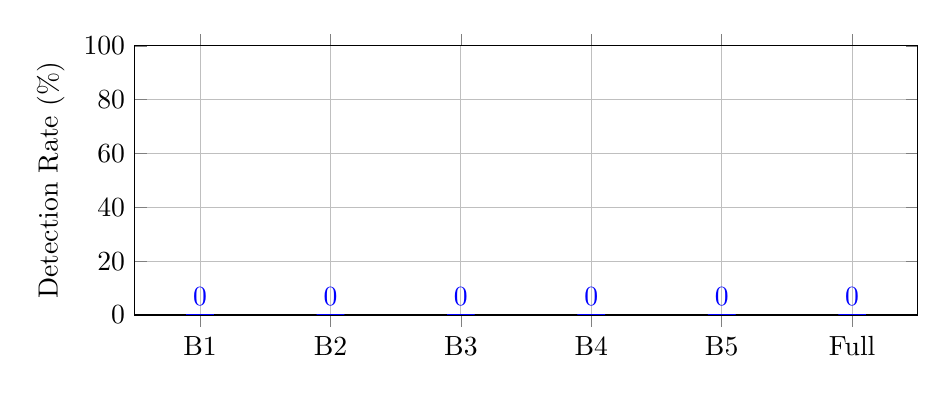
\begin{tikzpicture}
\begin{axis}[
    width=0.95\columnwidth,
    height=5cm,
    ybar,
    bar width=10pt,
    ymin=0, ymax=100,
    ylabel={Detection Rate (\%)},
    symbolic x coords={B1,B2,B3,B4,B5,Full},
    xtick=data,
    nodes near coords,
    grid=major
]
\addplot coordinates {(B1,0) (B2,0) (B3,0) (B4,0) (B5,0) (Full,0)};
\end{axis}
\end{tikzpicture}
\caption{Template for detection-rate comparison across baselines.}
\end{figure}

\subsection{Latency Comparison}
\begin{figure}[ht]
\centering
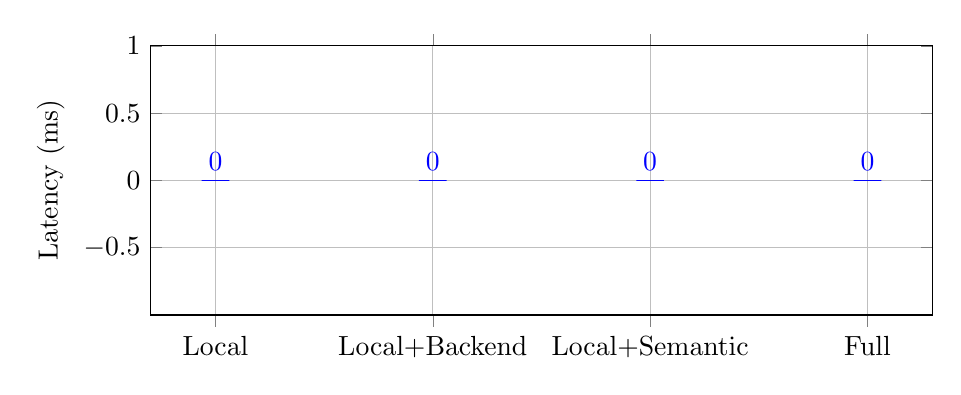
\begin{tikzpicture}
\begin{axis}[
    width=0.95\columnwidth,
    height=5cm,
    ybar,
    bar width=10pt,
    ymin=0,
    ylabel={Latency (ms)},
    symbolic x coords={Local,Local+Backend,Local+Semantic,Full},
    xtick=data,
    nodes near coords,
    grid=major
]
\addplot coordinates {(Local,0) (Local+Backend,0) (Local+Semantic,0) (Full,0)};
\end{axis}
\end{tikzpicture}
\caption{Template for latency overhead analysis.}
\end{figure}

\subsection{Ablation Plot}
\begin{figure}[ht]
\centering
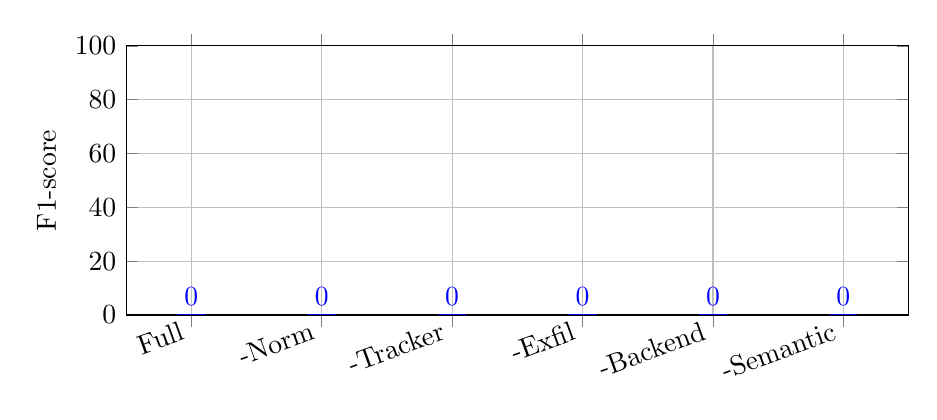
\begin{tikzpicture}
\begin{axis}[
    width=0.95\columnwidth,
    height=5cm,
    ybar,
    bar width=10pt,
    ymin=0, ymax=100,
    ylabel={F1-score},
    symbolic x coords={Full,-Norm,-Tracker,-Exfil,-Backend,-Semantic},
    xtick=data,
    x tick label style={rotate=20,anchor=east},
    nodes near coords,
    grid=major
]
\addplot coordinates {(Full,0) (-Norm,0) (-Tracker,0) (-Exfil,0) (-Backend,0) (-Semantic,0)};
\end{axis}
\end{tikzpicture}
\caption{Template for ablation study.}
\end{figure}

\section{Statistical Analysis Plan}
A complete journal study should report repeated-run averages, standard deviation, and confidence intervals. Pairwise comparison between the full system and baselines can be performed using paired tests on matched prompt sets. Bootstrapping is appropriate when the dataset contains heterogeneous attack categories.

\section{Discussion}
Gradril is strong as an architecture paper because the implementation already captures several practically relevant security ideas: normalization against obfuscation, modular local detection, optional ML-backed back-end validation, and domain-specific exfiltration checks. Its main strength is architectural specialization rather than a single large classifier.

The main limitation for journal publication is not architecture but evidence. The current draft is credible as a design and implementation paper, but journal reviewers will expect real measured results, more references, and stronger baseline comparison. Another limitation is that the semantic endpoint is implemented but not yet integrated into the active runtime path, and the local decision engine currently sanitizes rather than blocks.

\section{Conclusion}
Part III presented the benchmark design required to elevate Gradril from a strong architecture prototype to a full journal submission. With real datasets, measured metrics, ablations, and graphs inserted into the provided templates, the three-part split can be combined into a complete 15--20 page journal manuscript.

\begin{thebibliography}{9}
\bibitem{owasp_llm_top10}
OWASP Foundation, ``OWASP Top 10 for Large Language Model Applications,'' 2023.

\bibitem{greshake2023more}
K. Greshake et al., ``More than you've asked for: A comprehensive analysis of prompt injection threats,'' \textit{arXiv preprint arXiv:2302.12173}, 2023.

\bibitem{perez2022ignore}
F. Perez and I. Ribeiro, ``Ignore previous prompt: Attack techniques for language models,'' 2022.
\end{thebibliography}

\end{document}
